\documentclass[twoside]{book}

% Packages required by doxygen
\usepackage{calc}
\usepackage{doxygen}
\usepackage{graphicx}
\usepackage[utf8]{inputenc}
\usepackage{makeidx}
\usepackage{multicol}
\usepackage{multirow}
\usepackage{textcomp}
\usepackage[table]{xcolor}

% Font selection
\usepackage[T1]{fontenc}
\usepackage{mathptmx}
\usepackage[scaled=.90]{helvet}
\usepackage{courier}
\usepackage{amssymb}
\usepackage{sectsty}
\renewcommand{\familydefault}{\sfdefault}
\allsectionsfont{%
  \fontseries{bc}\selectfont%
  \color{darkgray}%
}
\renewcommand{\DoxyLabelFont}{%
  \fontseries{bc}\selectfont%
  \color{darkgray}%
}

% Page & text layout
\usepackage{geometry}
\geometry{%
  a4paper,%
  top=2.5cm,%
  bottom=2.5cm,%
  left=2.5cm,%
  right=2.5cm%
}
\tolerance=750
\hfuzz=15pt
\hbadness=750
\setlength{\emergencystretch}{15pt}
\setlength{\parindent}{0cm}
\setlength{\parskip}{0.2cm}
\makeatletter
\renewcommand{\paragraph}{%
  \@startsection{paragraph}{4}{0ex}{-1.0ex}{1.0ex}{%
    \normalfont\normalsize\bfseries\SS@parafont%
  }%
}
\renewcommand{\subparagraph}{%
  \@startsection{subparagraph}{5}{0ex}{-1.0ex}{1.0ex}{%
    \normalfont\normalsize\bfseries\SS@subparafont%
  }%
}
\makeatother

% Headers & footers
\usepackage{fancyhdr}
\pagestyle{fancyplain}
\fancyhead[LE]{\fancyplain{}{\bfseries\thepage}}
\fancyhead[CE]{\fancyplain{}{}}
\fancyhead[RE]{\fancyplain{}{\bfseries\leftmark}}
\fancyhead[LO]{\fancyplain{}{\bfseries\rightmark}}
\fancyhead[CO]{\fancyplain{}{}}
\fancyhead[RO]{\fancyplain{}{\bfseries\thepage}}
\fancyfoot[LE]{\fancyplain{}{}}
\fancyfoot[CE]{\fancyplain{}{}}
\fancyfoot[RE]{\fancyplain{}{\bfseries\scriptsize Generated on Sun Apr 19 2020 23\-:00\-:08 for Pitch Perfector by Doxygen }}
\fancyfoot[LO]{\fancyplain{}{\bfseries\scriptsize Generated on Sun Apr 19 2020 23\-:00\-:08 for Pitch Perfector by Doxygen }}
\fancyfoot[CO]{\fancyplain{}{}}
\fancyfoot[RO]{\fancyplain{}{}}
\renewcommand{\footrulewidth}{0.4pt}
\renewcommand{\chaptermark}[1]{%
  \markboth{#1}{}%
}
\renewcommand{\sectionmark}[1]{%
  \markright{\thesection\ #1}%
}

% Indices & bibliography
\usepackage{natbib}
\usepackage[titles]{tocloft}
\setcounter{tocdepth}{3}
\setcounter{secnumdepth}{5}
\makeindex

% Hyperlinks (required, but should be loaded last)
\usepackage{ifpdf}
\ifpdf
  \usepackage[pdftex,pagebackref=true]{hyperref}
\else
  \usepackage[ps2pdf,pagebackref=true]{hyperref}
\fi
\hypersetup{%
  colorlinks=true,%
  linkcolor=blue,%
  citecolor=blue,%
  unicode%
}

% Custom commands
\newcommand{\clearemptydoublepage}{%
  \newpage{\pagestyle{empty}\cleardoublepage}%
}


%===== C O N T E N T S =====

\begin{document}

% Titlepage & ToC
\hypersetup{pageanchor=false}
\pagenumbering{roman}
\begin{titlepage}
\vspace*{7cm}
\begin{center}%
{\Large Pitch Perfector }\\
\vspace*{1cm}
{\large Generated by Doxygen 1.8.6}\\
\vspace*{0.5cm}
{\small Sun Apr 19 2020 23:00:08}\\
\end{center}
\end{titlepage}
\clearemptydoublepage
\tableofcontents
\clearemptydoublepage
\pagenumbering{arabic}
\hypersetup{pageanchor=true}

%--- Begin generated contents ---
\chapter{Main Page}
\label{index}\hypertarget{index}{}The software for this project involves filtering, frequency analysis and pitch shifting.

For a description of the software design, see the project \href{https://github.com/a2198699s/pitch-perfector/wiki/Software-Design}{\tt Wiki}

The code is documented through \href{https://a2198699s.github.io/pitch-perfector/html/index.html}{\tt Doxygen}

The project is maintained on \href{https://github.com/a2198699s/pitch-perfector}{\tt Github}

Follow us on \href{https://twitter.com/PerfectorPitch}{\tt Twitter} and subscribe to our \href{https://www.youtube.com/channel/UCyVIknnXCnTIX-vixUphqTg}{\tt You\-Tube Channel} 
\chapter{Hierarchical Index}
\section{Class Hierarchy}
This inheritance list is sorted roughly, but not completely, alphabetically\-:\begin{DoxyCompactList}
\item \contentsline{section}{dispatch}{\pageref{classdispatch}}{}
\item \contentsline{section}{Dispatch}{\pageref{classDispatch}}{}
\item \contentsline{section}{fft}{\pageref{classfft}}{}
\item Q\-Thread\begin{DoxyCompactList}
\item \contentsline{section}{audio\-Streamer}{\pageref{classaudioStreamer}}{}
\end{DoxyCompactList}
\item Q\-Widget\begin{DoxyCompactList}
\item \contentsline{section}{Window}{\pageref{classWindow}}{}
\end{DoxyCompactList}
\item \contentsline{section}{Vocoder}{\pageref{classVocoder}}{}
\item \contentsline{section}{vocoder}{\pageref{classvocoder}}{}
\item \contentsline{section}{Vox\-Filter}{\pageref{classVoxFilter}}{}
\end{DoxyCompactList}

\chapter{Class Index}
\section{Class List}
Here are the classes, structs, unions and interfaces with brief descriptions\-:\begin{DoxyCompactList}
\item\contentsline{section}{\hyperlink{classaudioStreamer}{audio\-Streamer} }{\pageref{classaudioStreamer}}{}
\item\contentsline{section}{\hyperlink{classdispatch}{dispatch} \\*This class handles the callback functionality from Rt\-Audio }{\pageref{classdispatch}}{}
\item\contentsline{section}{\hyperlink{classDispatch}{Dispatch} }{\pageref{classDispatch}}{}
\item\contentsline{section}{\hyperlink{classfft}{fft} \\*Class for performing fourier transforms using F\-F\-T\-W3 }{\pageref{classfft}}{}
\item\contentsline{section}{\hyperlink{classVocoder}{Vocoder} }{\pageref{classVocoder}}{}
\item\contentsline{section}{\hyperlink{classvocoder}{vocoder} }{\pageref{classvocoder}}{}
\item\contentsline{section}{\hyperlink{classWindow}{Window} }{\pageref{classWindow}}{}
\end{DoxyCompactList}

\chapter{Class Documentation}
\hypertarget{classaudioStreamer}{\section{audio\-Streamer Class Reference}
\label{classaudioStreamer}\index{audio\-Streamer@{audio\-Streamer}}
}
Inheritance diagram for audio\-Streamer\-:\begin{figure}[H]
\begin{center}
\leavevmode
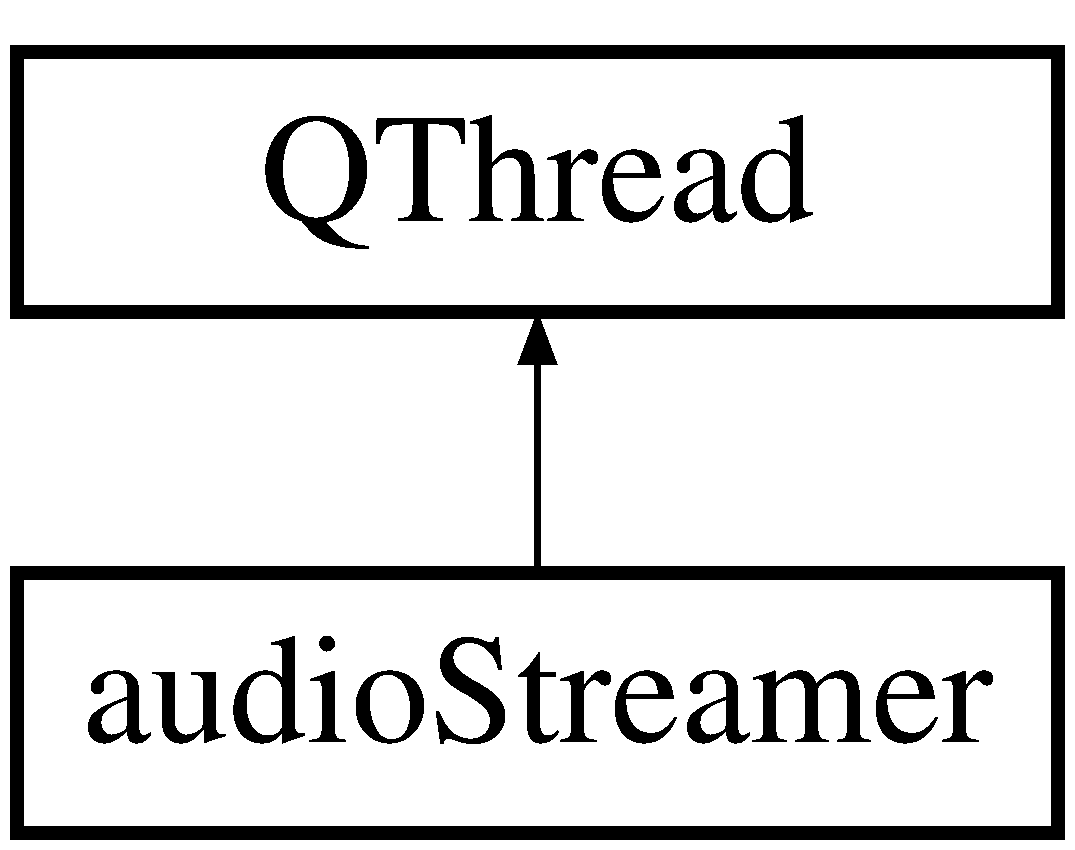
\includegraphics[height=2.000000cm]{classaudioStreamer}
\end{center}
\end{figure}
\subsection*{Public Member Functions}
\begin{DoxyCompactItemize}
\item 
\hypertarget{classaudioStreamer_aa236fda0774b738734c2c62b92a912c3}{void {\bfseries quit} ()}\label{classaudioStreamer_aa236fda0774b738734c2c62b92a912c3}

\item 
\hypertarget{classaudioStreamer_a7488bec15fe99d666b66dd5fa45df74e}{void {\bfseries run} ()}\label{classaudioStreamer_a7488bec15fe99d666b66dd5fa45df74e}

\item 
\hypertarget{classaudioStreamer_aa236fda0774b738734c2c62b92a912c3}{void {\bfseries quit} ()}\label{classaudioStreamer_aa236fda0774b738734c2c62b92a912c3}

\item 
\hypertarget{classaudioStreamer_a7488bec15fe99d666b66dd5fa45df74e}{void {\bfseries run} ()}\label{classaudioStreamer_a7488bec15fe99d666b66dd5fa45df74e}

\end{DoxyCompactItemize}
\subsection*{Public Attributes}
\begin{DoxyCompactItemize}
\item 
\hypertarget{classaudioStreamer_a392bb08783c92e356e704f40ff6a109a}{double $\ast$ {\bfseries input\-Data}}\label{classaudioStreamer_a392bb08783c92e356e704f40ff6a109a}

\item 
\hypertarget{classaudioStreamer_ab44575639696ec28e58a0ca4d5e7d099}{fftw\-\_\-complex $\ast$ {\bfseries output\-Data}}\label{classaudioStreamer_ab44575639696ec28e58a0ca4d5e7d099}

\item 
\hypertarget{classaudioStreamer_a1d8289cf32dd73375172f06c998d7a9f}{double $\ast$ {\bfseries inverse\-Out}}\label{classaudioStreamer_a1d8289cf32dd73375172f06c998d7a9f}

\item 
\hypertarget{classaudioStreamer_a02267d0dc3b957a812327cd56299c459}{float $\ast$ {\bfseries distance\-To\-Note}}\label{classaudioStreamer_a02267d0dc3b957a812327cd56299c459}

\item 
\hypertarget{classaudioStreamer_a943371f31102ab0f493addfbd685f210}{char $\ast$ {\bfseries current\-Note}}\label{classaudioStreamer_a943371f31102ab0f493addfbd685f210}

\item 
\hypertarget{classaudioStreamer_a721e16ff965429808516f39e93c50b82}{double {\bfseries current\-Note}}\label{classaudioStreamer_a721e16ff965429808516f39e93c50b82}

\end{DoxyCompactItemize}


The documentation for this class was generated from the following files\-:\begin{DoxyCompactItemize}
\item 
/home/travis/build/a2198699s/pitch-\/perfector/\-Code/fft\-\_\-object/audio\-Streamer.\-h\item 
/home/travis/build/a2198699s/pitch-\/perfector/\-Code/fft\-\_\-object/audio\-Streamer.\-cpp\end{DoxyCompactItemize}

\hypertarget{classdispatch}{\section{dispatch Class Reference}
\label{classdispatch}\index{dispatch@{dispatch}}
}
\subsection*{Public Member Functions}
\begin{DoxyCompactItemize}
\item 
\hypertarget{classdispatch_a641ec1136a8fdecb8b9ab51fa672a848}{{\bfseries dispatch} (\hyperlink{classfft}{fft} $\ast$fourier\-Ptr, \hyperlink{classvocoder}{vocoder} $\ast$vocoder\-Ptr)}\label{classdispatch_a641ec1136a8fdecb8b9ab51fa672a848}

\item 
\hypertarget{classdispatch_a49638cdbc0fee44e411973f09fc64d83}{{\bfseries dispatch} (\hyperlink{classfft}{fft} $\ast$fourier\-\_\-obj, \hyperlink{classvocoder}{vocoder} $\ast$vocoder\-\_\-obj)}\label{classdispatch_a49638cdbc0fee44e411973f09fc64d83}

\item 
\hypertarget{classdispatch_a49638cdbc0fee44e411973f09fc64d83}{{\bfseries dispatch} (\hyperlink{classfft}{fft} $\ast$fourier\-\_\-obj, \hyperlink{classvocoder}{vocoder} $\ast$vocoder\-\_\-obj)}\label{classdispatch_a49638cdbc0fee44e411973f09fc64d83}

\end{DoxyCompactItemize}
\subsection*{Static Public Member Functions}
\begin{DoxyCompactItemize}
\item 
\hypertarget{classdispatch_a78e0b45ddb573d1b843ce02cd9092557}{static int {\bfseries caller} (void $\ast$output\-Buffer, void $\ast$input\-Buffer, unsigned int n\-Buffer\-Frames, double stream\-Time, Rt\-Audio\-Stream\-Status status, void $\ast$data)}\label{classdispatch_a78e0b45ddb573d1b843ce02cd9092557}

\item 
\hypertarget{classdispatch_a2bc93711c1aee895c430aece41ec026a}{static int {\bfseries caller} (void $\ast$output\-Buffer, void $\ast$input\-Buffer, unsigned int n\-Buffer\-Frames, double stream\-Time, Rt\-Audio\-Stream\-Status status, void $\ast$data)}\label{classdispatch_a2bc93711c1aee895c430aece41ec026a}

\item 
\hypertarget{classdispatch_a2bc93711c1aee895c430aece41ec026a}{static int {\bfseries caller} (void $\ast$output\-Buffer, void $\ast$input\-Buffer, unsigned int n\-Buffer\-Frames, double stream\-Time, Rt\-Audio\-Stream\-Status status, void $\ast$data)}\label{classdispatch_a2bc93711c1aee895c430aece41ec026a}

\item 
\hypertarget{classdispatch_a2bc93711c1aee895c430aece41ec026a}{static int {\bfseries caller} (void $\ast$output\-Buffer, void $\ast$input\-Buffer, unsigned int n\-Buffer\-Frames, double stream\-Time, Rt\-Audio\-Stream\-Status status, void $\ast$data)}\label{classdispatch_a2bc93711c1aee895c430aece41ec026a}

\end{DoxyCompactItemize}
\subsection*{Public Attributes}
\begin{DoxyCompactItemize}
\item 
\hypertarget{classdispatch_a7b449abb93c0499530bec56afe866f5a}{\hyperlink{classfft}{fft} $\ast$ {\bfseries fourier\-Obj}}\label{classdispatch_a7b449abb93c0499530bec56afe866f5a}

\item 
\hypertarget{classdispatch_a7ccec21b2dce1224744ccaa8d1cafee5}{\hyperlink{classvocoder}{vocoder} $\ast$ {\bfseries vocoder\-Obj}}\label{classdispatch_a7ccec21b2dce1224744ccaa8d1cafee5}

\item 
\hypertarget{classdispatch_a25afc54bd990f1169d9fa75dc304793b}{\hyperlink{classfft}{fft} $\ast$ {\bfseries fourier\-Ptr}}\label{classdispatch_a25afc54bd990f1169d9fa75dc304793b}

\item 
\hypertarget{classdispatch_adf89bdb854ef17a8927bf7c506bfdc23}{\hyperlink{classvocoder}{vocoder} $\ast$ {\bfseries vocode\-Ptr}}\label{classdispatch_adf89bdb854ef17a8927bf7c506bfdc23}

\end{DoxyCompactItemize}


The documentation for this class was generated from the following files\-:\begin{DoxyCompactItemize}
\item 
/home/travis/build/a2198699s/pitch-\/perfector/\-Code/classfiles/dispatch.\-h\item 
/home/travis/build/a2198699s/pitch-\/perfector/\-Code/old/vocoder/vocoding.\-cpp\item 
/home/travis/build/a2198699s/pitch-\/perfector/\-Code/old/unknown/duplex\-\_\-fft/duplex\-\_\-obj.\-cpp\item 
/home/travis/build/a2198699s/pitch-\/perfector/\-Code/classfiles/dispatch.\-cpp\end{DoxyCompactItemize}

\hypertarget{classDispatch}{\section{Dispatch Class Reference}
\label{classDispatch}\index{Dispatch@{Dispatch}}
}
\subsection*{Static Public Member Functions}
\begin{DoxyCompactItemize}
\item 
\hypertarget{classDispatch_a53ca7df90385512d941a0b4cca324661}{static int {\bfseries caller} (void $\ast$output\-Buffer, void $\ast$input\-Buffer, unsigned int n\-Buffer\-Frames, double stream\-Time, Rt\-Audio\-Stream\-Status status, void $\ast$data)}\label{classDispatch_a53ca7df90385512d941a0b4cca324661}

\end{DoxyCompactItemize}


The documentation for this class was generated from the following files\-:\begin{DoxyCompactItemize}
\item 
/home/travis/build/a2198699s/pitch-\/perfector/\-Code/oopvocoder/fft.\-h\item 
/home/travis/build/a2198699s/pitch-\/perfector/\-Code/oopvocoder/fft.\-cpp\end{DoxyCompactItemize}

\hypertarget{classfft}{\section{fft Class Reference}
\label{classfft}\index{fft@{fft}}
}


Class for performing fourier transforms using F\-F\-T\-W3.  




{\ttfamily \#include $<$fft.\-h$>$}

\subsection*{Public Member Functions}
\begin{DoxyCompactItemize}
\item 
\hypertarget{classfft_a5fff94ac07119207ddd05f628be5891d}{\hyperlink{classfft_a5fff94ac07119207ddd05f628be5891d}{fft} (int n\-Buffer\-Frames)}\label{classfft_a5fff94ac07119207ddd05f628be5891d}

\begin{DoxyCompactList}\small\item\em Construct the fftw3 plans for the object. \end{DoxyCompactList}\item 
void \hyperlink{classfft_a47e58fd4f715ad89a6fad8df9d715bf4}{executefft} (double $\ast$input\-Buffer)
\item 
void \hyperlink{classfft_a228bd861564c189cd7b6800c950a1c09}{execute\-Inverse\-\_\-fft} (fftw\-\_\-complex $\ast$fourier\-Spectrum)
\item 
\hypertarget{classfft_a57f8fc9224851c0a827b3d46102f1623}{{\bfseries fft} (int n\-Buffer\-Frames, int sampling\-Rate)}\label{classfft_a57f8fc9224851c0a827b3d46102f1623}

\item 
\hypertarget{classfft_a47e58fd4f715ad89a6fad8df9d715bf4}{void {\bfseries executefft} (double $\ast$input\-Buffer)}\label{classfft_a47e58fd4f715ad89a6fad8df9d715bf4}

\item 
\hypertarget{classfft_a228bd861564c189cd7b6800c950a1c09}{void {\bfseries execute\-Inverse\-\_\-fft} (fftw\-\_\-complex $\ast$fourier\-Spectrum)}\label{classfft_a228bd861564c189cd7b6800c950a1c09}

\item 
\hypertarget{classfft_a57f8fc9224851c0a827b3d46102f1623}{\hyperlink{classfft_a57f8fc9224851c0a827b3d46102f1623}{fft} (int n\-Buffer\-Frames, int sampling\-Rate)}\label{classfft_a57f8fc9224851c0a827b3d46102f1623}

\begin{DoxyCompactList}\small\item\em Construct the fftw3 plans for the object. \end{DoxyCompactList}\item 
void \hyperlink{classfft_a47e58fd4f715ad89a6fad8df9d715bf4}{executefft} (double $\ast$input\-Buffer)
\item 
void \hyperlink{classfft_a228bd861564c189cd7b6800c950a1c09}{execute\-Inverse\-\_\-fft} (fftw\-\_\-complex $\ast$fourier\-Spectrum)
\item 
\hypertarget{classfft_a5fff94ac07119207ddd05f628be5891d}{{\bfseries fft} (int n\-Buffer\-Frames)}\label{classfft_a5fff94ac07119207ddd05f628be5891d}

\item 
\hypertarget{classfft_a47e58fd4f715ad89a6fad8df9d715bf4}{void {\bfseries executefft} (double $\ast$input\-Buffer)}\label{classfft_a47e58fd4f715ad89a6fad8df9d715bf4}

\item 
\hypertarget{classfft_a5fff94ac07119207ddd05f628be5891d}{{\bfseries fft} (int n\-Buffer\-Frames)}\label{classfft_a5fff94ac07119207ddd05f628be5891d}

\item 
\hypertarget{classfft_a47e58fd4f715ad89a6fad8df9d715bf4}{void {\bfseries executefft} (double $\ast$input\-Buffer)}\label{classfft_a47e58fd4f715ad89a6fad8df9d715bf4}

\item 
\hypertarget{classfft_a228bd861564c189cd7b6800c950a1c09}{void {\bfseries execute\-Inverse\-\_\-fft} (fftw\-\_\-complex $\ast$fourier\-Spectrum)}\label{classfft_a228bd861564c189cd7b6800c950a1c09}

\item 
\hypertarget{classfft_a5fff94ac07119207ddd05f628be5891d}{{\bfseries fft} (int n\-Buffer\-Frames)}\label{classfft_a5fff94ac07119207ddd05f628be5891d}

\item 
\hypertarget{classfft_a47e58fd4f715ad89a6fad8df9d715bf4}{void {\bfseries executefft} (double $\ast$input\-Buffer)}\label{classfft_a47e58fd4f715ad89a6fad8df9d715bf4}

\item 
\hypertarget{classfft_a228bd861564c189cd7b6800c950a1c09}{void {\bfseries execute\-Inverse\-\_\-fft} (fftw\-\_\-complex $\ast$fourier\-Spectrum)}\label{classfft_a228bd861564c189cd7b6800c950a1c09}

\end{DoxyCompactItemize}
\subsection*{Public Attributes}
\begin{DoxyCompactItemize}
\item 
\hypertarget{classfft_ab960a894180e634d2eace4b68700dff3}{int {\bfseries n\-Buffer\-Frames}}\label{classfft_ab960a894180e634d2eace4b68700dff3}

\item 
\hypertarget{classfft_ad52a575c3cf3f7aae014927bcc4cbbe2}{double $\ast$ {\bfseries in}}\label{classfft_ad52a575c3cf3f7aae014927bcc4cbbe2}

\item 
\hypertarget{classfft_a21e2e595b77d7f003ec24075eb892fe1}{fftw\-\_\-complex $\ast$ {\bfseries out}}\label{classfft_a21e2e595b77d7f003ec24075eb892fe1}

\item 
\hypertarget{classfft_a30b05b794baa0c8965b7e4cc63bafd98}{fftw\-\_\-complex $\ast$ {\bfseries inverse\-\_\-in}}\label{classfft_a30b05b794baa0c8965b7e4cc63bafd98}

\item 
\hypertarget{classfft_a162e76aaf4e73ff332cd71f81556fbcc}{double $\ast$ {\bfseries inverse\-\_\-out}}\label{classfft_a162e76aaf4e73ff332cd71f81556fbcc}

\item 
\hypertarget{classfft_a2845f6a00618246fc6adfb57ae106925}{fftw\-\_\-plan {\bfseries my\-\_\-plan}}\label{classfft_a2845f6a00618246fc6adfb57ae106925}

\item 
\hypertarget{classfft_a8b7b6b88eb0b9aaf7ae7580e5b42a533}{fftw\-\_\-plan {\bfseries inverse\-\_\-plan}}\label{classfft_a8b7b6b88eb0b9aaf7ae7580e5b42a533}

\item 
\hypertarget{classfft_ad7bd6dde9d599f62bd764ad986ac4305}{double {\bfseries in} \mbox{[}A\-U\-D\-I\-O\-\_\-\-B\-U\-F\-F\-E\-R\-\_\-\-S\-I\-Z\-E\mbox{]}}\label{classfft_ad7bd6dde9d599f62bd764ad986ac4305}

\item 
\hypertarget{classfft_a6c30ac336ab818e27c0a819ad942a6f3}{fftw\-\_\-complex {\bfseries out} \mbox{[}F\-F\-T\-\_\-\-B\-U\-F\-F\-E\-R\-\_\-\-S\-I\-Z\-E\mbox{]}}\label{classfft_a6c30ac336ab818e27c0a819ad942a6f3}

\item 
\hypertarget{classfft_adc3213de8e941a184c2ec3a1ca31815a}{fftw\-\_\-complex {\bfseries inverse\-\_\-in} \mbox{[}F\-F\-T\-\_\-\-B\-U\-F\-F\-E\-R\-\_\-\-S\-I\-Z\-E\mbox{]}}\label{classfft_adc3213de8e941a184c2ec3a1ca31815a}

\item 
\hypertarget{classfft_a290d4177db41a835118d5e0003ec7e2f}{double {\bfseries inverse\-\_\-out} \mbox{[}A\-U\-D\-I\-O\-\_\-\-B\-U\-F\-F\-E\-R\-\_\-\-S\-I\-Z\-E\mbox{]}}\label{classfft_a290d4177db41a835118d5e0003ec7e2f}

\item 
\hypertarget{classfft_add70853a9fc0ac681a974a8e1a40dfd8}{int {\bfseries sampling\-Rate}}\label{classfft_add70853a9fc0ac681a974a8e1a40dfd8}

\item 
\hypertarget{classfft_a3eda9964a8016b8683b5b5581fb90636}{\hyperlink{classVoxFilter}{Vox\-Filter} $\ast$ {\bfseries vox\-Filter}}\label{classfft_a3eda9964a8016b8683b5b5581fb90636}

\item 
\hypertarget{classfft_a46fd389fd4116e85af557fd191326586}{\hyperlink{classVoxFilter}{Vox\-Filter} $\ast$ {\bfseries vfilter}}\label{classfft_a46fd389fd4116e85af557fd191326586}

\item 
\hypertarget{classfft_a66afecdbae4bef314698644fc3f280de}{int {\bfseries flag}}\label{classfft_a66afecdbae4bef314698644fc3f280de}

\end{DoxyCompactItemize}


\subsection{Detailed Description}
Class for performing fourier transforms using F\-F\-T\-W3. 

Allows for the set-\/up of a fftw3 plan (the most time consuming part of the process) when the class instantiated, allowing the performance of forward and inverse fast fourier transforms with minimal computational cost inside the Rt\-Audio Callback when the methods are called. 

\subsection{Member Function Documentation}
\hypertarget{classfft_a47e58fd4f715ad89a6fad8df9d715bf4}{\index{fft@{fft}!executefft@{executefft}}
\index{executefft@{executefft}!fft@{fft}}
\subsubsection[{executefft}]{\setlength{\rightskip}{0pt plus 5cm}void fft\-::executefft (
\begin{DoxyParamCaption}
\item[{double $\ast$}]{input\-Buffer}
\end{DoxyParamCaption}
)}}\label{classfft_a47e58fd4f715ad89a6fad8df9d715bf4}
Execute the forward fourier transform and update generate the frequncy spectrum for the data input \hypertarget{classfft_a47e58fd4f715ad89a6fad8df9d715bf4}{\index{fft@{fft}!executefft@{executefft}}
\index{executefft@{executefft}!fft@{fft}}
\subsubsection[{executefft}]{\setlength{\rightskip}{0pt plus 5cm}void fft\-::executefft (
\begin{DoxyParamCaption}
\item[{double $\ast$}]{input\-Buffer}
\end{DoxyParamCaption}
)}}\label{classfft_a47e58fd4f715ad89a6fad8df9d715bf4}
Execute the forward fourier transform and update generate the frequncy spectrum for the data input \hypertarget{classfft_a228bd861564c189cd7b6800c950a1c09}{\index{fft@{fft}!execute\-Inverse\-\_\-fft@{execute\-Inverse\-\_\-fft}}
\index{execute\-Inverse\-\_\-fft@{execute\-Inverse\-\_\-fft}!fft@{fft}}
\subsubsection[{execute\-Inverse\-\_\-fft}]{\setlength{\rightskip}{0pt plus 5cm}void fft\-::execute\-Inverse\-\_\-fft (
\begin{DoxyParamCaption}
\item[{fftw\-\_\-complex $\ast$}]{fourier\-Spectrum}
\end{DoxyParamCaption}
)}}\label{classfft_a228bd861564c189cd7b6800c950a1c09}
Execute the inverse fourier transform to reconstruct a time-\/series signal from the input frequency spectrum. Data is then scaled back to the appropriate size. \hypertarget{classfft_a228bd861564c189cd7b6800c950a1c09}{\index{fft@{fft}!execute\-Inverse\-\_\-fft@{execute\-Inverse\-\_\-fft}}
\index{execute\-Inverse\-\_\-fft@{execute\-Inverse\-\_\-fft}!fft@{fft}}
\subsubsection[{execute\-Inverse\-\_\-fft}]{\setlength{\rightskip}{0pt plus 5cm}void fft\-::execute\-Inverse\-\_\-fft (
\begin{DoxyParamCaption}
\item[{fftw\-\_\-complex $\ast$}]{fourier\-Spectrum}
\end{DoxyParamCaption}
)}}\label{classfft_a228bd861564c189cd7b6800c950a1c09}
Execute the inverse fourier transform to reconstruct a time-\/series signal from the input frequency spectrum. Data is then scaled back to the appropriate size. 

The documentation for this class was generated from the following files\-:\begin{DoxyCompactItemize}
\item 
/home/travis/build/a2198699s/pitch-\/perfector/\-Code/classfiles/fft.\-h\item 
/home/travis/build/a2198699s/pitch-\/perfector/\-Code/oopvocoder/vocoding.\-cpp\item 
/home/travis/build/a2198699s/pitch-\/perfector/\-Code/classfiles/fft.\-cpp\end{DoxyCompactItemize}

\hypertarget{classVocoder}{\section{Vocoder Class Reference}
\label{classVocoder}\index{Vocoder@{Vocoder}}
}
\subsection*{Public Member Functions}
\begin{DoxyCompactItemize}
\item 
\hypertarget{classVocoder_a3b1ed9bc5de7892f86bd2673ce72fd6e}{{\bfseries Vocoder} (int sample\-Rate, int buffer\-Size, const double $\ast$scale\-Frequencies)}\label{classVocoder_a3b1ed9bc5de7892f86bd2673ce72fd6e}

\item 
\hypertarget{classVocoder_a19c3f81b8451356f34601b6354e6d53e}{float {\bfseries binary\-\_\-search} (const float $\ast$Notes\-In\-Key, float $\ast$note, int highest\-\_\-index, int lowest\-\_\-index)}\label{classVocoder_a19c3f81b8451356f34601b6354e6d53e}

\item 
\hypertarget{classVocoder_a52ea6ca3fa19f44bdbbacf07e0e72064}{float {\bfseries note\-Finder} (const float $\ast$Notes\-In\-Key, float $\ast$note)}\label{classVocoder_a52ea6ca3fa19f44bdbbacf07e0e72064}

\item 
\hypertarget{classVocoder_a6ac34c186396037e8546fd03b5a0b51a}{float {\bfseries Sample\-To\-Freq} (int sample)}\label{classVocoder_a6ac34c186396037e8546fd03b5a0b51a}

\item 
\hypertarget{classVocoder_a205b461f0bf7c3b1ffb0b8a89ccd5e72}{void {\bfseries pitch\-Shift\-\_\-setup} (fftw\-\_\-complex $\ast$fft\-\_\-spectrum)}\label{classVocoder_a205b461f0bf7c3b1ffb0b8a89ccd5e72}

\item 
\hypertarget{classVocoder_a31c2f03502edb92a86ce799fbf4957f6}{void {\bfseries pitch\-Shift} ()}\label{classVocoder_a31c2f03502edb92a86ce799fbf4957f6}

\item 
\hypertarget{classVocoder_ad7e75d0c54cb9d2b1eb8f077050a6f81}{void {\bfseries find\-Peak} ()}\label{classVocoder_ad7e75d0c54cb9d2b1eb8f077050a6f81}

\item 
\hypertarget{classVocoder_ab736b53577e9ba92259a5c4074a0bf00}{double {\bfseries get\-Closest} (double val1, double val2, double target)}\label{classVocoder_ab736b53577e9ba92259a5c4074a0bf00}

\item 
\hypertarget{classVocoder_a0bc26c9977b46623e3c3fc3bc733ed24}{double {\bfseries find\-Closest\-Note} (const double notes\mbox{[}$\,$\mbox{]}, int n, double target)}\label{classVocoder_a0bc26c9977b46623e3c3fc3bc733ed24}

\item 
\hypertarget{classVocoder_aae99cff1d3e7fc029433998dc7fd0381}{int {\bfseries Frequency\-To\-Index} (double frequency)}\label{classVocoder_aae99cff1d3e7fc029433998dc7fd0381}

\item 
\hypertarget{classVocoder_a223d77b73ef3b2fa8be406e46f671441}{void {\bfseries set\-Fourier\-Spectrum} (fftw\-\_\-complex $\ast$fft\-Spectrum)}\label{classVocoder_a223d77b73ef3b2fa8be406e46f671441}

\item 
\hypertarget{classVocoder_a4fd5417891ffeb5668dc9c52478c2428}{const char $\ast$ {\bfseries frequency\-To\-Note} (double freq)}\label{classVocoder_a4fd5417891ffeb5668dc9c52478c2428}

\item 
\hypertarget{classVocoder_aee9e5b1265e55d99488164f4a9527d65}{char $\ast$ {\bfseries get\-Note} ()}\label{classVocoder_aee9e5b1265e55d99488164f4a9527d65}

\end{DoxyCompactItemize}
\subsection*{Public Attributes}
\begin{DoxyCompactItemize}
\item 
\hypertarget{classVocoder_a47e8c37097fafbe8bd8a87adba84e5f1}{float {\bfseries base\-Freq}}\label{classVocoder_a47e8c37097fafbe8bd8a87adba84e5f1}

\item 
\hypertarget{classVocoder_ad4f1e12813090bb2a980be7aa3bac471}{int {\bfseries base\-Sample}}\label{classVocoder_ad4f1e12813090bb2a980be7aa3bac471}

\item 
\hypertarget{classVocoder_a7fa47ae2edf71aeb5b36e875bb440667}{int {\bfseries samplerate}}\label{classVocoder_a7fa47ae2edf71aeb5b36e875bb440667}

\item 
\hypertarget{classVocoder_a38c9aa4fad739f7577e51fc3d4891751}{int {\bfseries buffer\-Size}}\label{classVocoder_a38c9aa4fad739f7577e51fc3d4891751}

\item 
\hypertarget{classVocoder_a5bd2da8b9a6b618be7828035dfb50f53}{float {\bfseries frequency\-Resolution}}\label{classVocoder_a5bd2da8b9a6b618be7828035dfb50f53}

\item 
\hypertarget{classVocoder_a2cf377a9138da30b22b273f55915ea65}{const double $\ast$ {\bfseries scale\-Frequencies}}\label{classVocoder_a2cf377a9138da30b22b273f55915ea65}

\item 
\hypertarget{classVocoder_a77dcc19311b4905125bf609084b4ad2a}{float {\bfseries new\-Freq}}\label{classVocoder_a77dcc19311b4905125bf609084b4ad2a}

\item 
\hypertarget{classVocoder_a300f616506453a971cf21a7de35e2964}{float {\bfseries difference}}\label{classVocoder_a300f616506453a971cf21a7de35e2964}

\item 
\hypertarget{classVocoder_acd33a5938c9167429b2a4cd8c58374ae}{int {\bfseries bin\-Difference}}\label{classVocoder_acd33a5938c9167429b2a4cd8c58374ae}

\item 
\hypertarget{classVocoder_a2884b2fe7d5303609ddeff6979bdbcd3}{fftw\-\_\-complex {\bfseries fourier\-Spectrum} \mbox{[}257\mbox{]}}\label{classVocoder_a2884b2fe7d5303609ddeff6979bdbcd3}

\item 
\hypertarget{classVocoder_abae7bb20fa180d030d6a96f08af48429}{double {\bfseries peak\-Frequency}}\label{classVocoder_abae7bb20fa180d030d6a96f08af48429}

\item 
\hypertarget{classVocoder_a6550fbf8de5847c7d5a6fcb90b4f3c2b}{double {\bfseries closest\-Note\-Frequency}}\label{classVocoder_a6550fbf8de5847c7d5a6fcb90b4f3c2b}

\item 
\hypertarget{classVocoder_acdf99dd6f1b47d1bcf539c87b1500c56}{char {\bfseries current\-Note} \mbox{[}2\mbox{]}}\label{classVocoder_acdf99dd6f1b47d1bcf539c87b1500c56}

\end{DoxyCompactItemize}


The documentation for this class was generated from the following files\-:\begin{DoxyCompactItemize}
\item 
/home/travis/build/a2198699s/pitch-\/perfector/\-Code/fft\-\_\-object/vocoder.\-h\item 
/home/travis/build/a2198699s/pitch-\/perfector/\-Code/fft\-\_\-object/vocoder.\-cpp\end{DoxyCompactItemize}

\hypertarget{classvocoder}{\section{vocoder Class Reference}
\label{classvocoder}\index{vocoder@{vocoder}}
}


{\ttfamily \#include $<$vocoder.\-h$>$}

\subsection*{Public Member Functions}
\begin{DoxyCompactItemize}
\item 
\hypertarget{classvocoder_a5e51f2bff73fdb41cb326e0743170b15}{{\bfseries vocoder} (int samplerate\-\_\-input, int buffer\-Size\-\_\-input, const float $\ast$scale\-Freqs\-\_\-input)}\label{classvocoder_a5e51f2bff73fdb41cb326e0743170b15}

\item 
\hypertarget{classvocoder_a516a5e099509664b6b328a9d055adcd7}{float {\bfseries binary\-\_\-search} (const float $\ast$Notes\-In\-Key, float $\ast$note, int highest\-\_\-index, int lowest\-\_\-index)}\label{classvocoder_a516a5e099509664b6b328a9d055adcd7}

\item 
\hypertarget{classvocoder_ac1c52677bdf6c7233f667c3905539716}{float {\bfseries note\-Finder} (const float $\ast$Notes\-In\-Key, float $\ast$note)}\label{classvocoder_ac1c52677bdf6c7233f667c3905539716}

\item 
\hypertarget{classvocoder_a2b3a6e386d3a18f9366320e5743d33b1}{float {\bfseries Sample\-To\-Freq} (int sample)}\label{classvocoder_a2b3a6e386d3a18f9366320e5743d33b1}

\item 
void \hyperlink{classvocoder_aa3d122aee6d6ae77ac5b04572e924dc0}{pitch\-Shift\-\_\-setup} (fftw\-\_\-complex $\ast$fft\-\_\-spectrum)
\item 
\hypertarget{classvocoder_aa218678a51da7429066c32e59edd5057}{void {\bfseries pitch\-Shift} ()}\label{classvocoder_aa218678a51da7429066c32e59edd5057}

\item 
\hypertarget{classvocoder_a5e51f2bff73fdb41cb326e0743170b15}{{\bfseries vocoder} (int samplerate\-\_\-input, int buffer\-Size\-\_\-input, const float $\ast$scale\-Freqs\-\_\-input)}\label{classvocoder_a5e51f2bff73fdb41cb326e0743170b15}

\item 
\hypertarget{classvocoder_a7a0b1f788e03878de287d7f6163208a9}{float {\bfseries binary\-\_\-search} (const float $\ast$Notes\-In\-Key, float $\ast$note, int highest\-\_\-index, int lowest\-\_\-index)}\label{classvocoder_a7a0b1f788e03878de287d7f6163208a9}

\item 
\hypertarget{classvocoder_afb731a113935c575939ebdff7ae37580}{float {\bfseries note\-Finder} (const float $\ast$Notes\-In\-Key, float $\ast$note)}\label{classvocoder_afb731a113935c575939ebdff7ae37580}

\item 
\hypertarget{classvocoder_a2b3a6e386d3a18f9366320e5743d33b1}{float {\bfseries Sample\-To\-Freq} (int sample)}\label{classvocoder_a2b3a6e386d3a18f9366320e5743d33b1}

\item 
\hypertarget{classvocoder_aa3d122aee6d6ae77ac5b04572e924dc0}{void {\bfseries pitch\-Shift\-\_\-setup} (fftw\-\_\-complex $\ast$fft\-\_\-spectrum)}\label{classvocoder_aa3d122aee6d6ae77ac5b04572e924dc0}

\item 
\hypertarget{classvocoder_aa218678a51da7429066c32e59edd5057}{void {\bfseries pitch\-Shift} ()}\label{classvocoder_aa218678a51da7429066c32e59edd5057}

\item 
\hypertarget{classvocoder_a759189527108a2f32b992406b8210db8}{{\bfseries vocoder} (int samplerate\-\_\-input, int buffer\-Size\-\_\-input, void $\ast$scale\-Freqs\-\_\-input)}\label{classvocoder_a759189527108a2f32b992406b8210db8}

\item 
\hypertarget{classvocoder_a2b3a6e386d3a18f9366320e5743d33b1}{float {\bfseries Sample\-To\-Freq} (int sample)}\label{classvocoder_a2b3a6e386d3a18f9366320e5743d33b1}

\item 
\hypertarget{classvocoder_a8b1e51e28458338abc0eeaac00c1842f}{int {\bfseries Nearest\-Note} (float $\ast$freq)}\label{classvocoder_a8b1e51e28458338abc0eeaac00c1842f}

\item 
\hypertarget{classvocoder_aa3d122aee6d6ae77ac5b04572e924dc0}{void {\bfseries pitch\-Shift\-\_\-setup} (fftw\-\_\-complex $\ast$fft\-\_\-spectrum)}\label{classvocoder_aa3d122aee6d6ae77ac5b04572e924dc0}

\item 
\hypertarget{classvocoder_aa218678a51da7429066c32e59edd5057}{void {\bfseries pitch\-Shift} ()}\label{classvocoder_aa218678a51da7429066c32e59edd5057}

\end{DoxyCompactItemize}
\subsection*{Static Public Member Functions}
\begin{DoxyCompactItemize}
\item 
\hypertarget{classvocoder_a54dbb5d460704f880382d2ae7e64e14a}{static int {\bfseries binary\-\_\-search} (const float $\ast$Notes\-In\-Key, float $\ast$note, int highest\-\_\-index, int lowest\-\_\-index)}\label{classvocoder_a54dbb5d460704f880382d2ae7e64e14a}

\item 
\hypertarget{classvocoder_a450b5c7824587e81db5aa4c056ba6934}{static int {\bfseries note\-Finder} (const float $\ast$Notes\-In\-Key, float $\ast$note)}\label{classvocoder_a450b5c7824587e81db5aa4c056ba6934}

\end{DoxyCompactItemize}
\subsection*{Public Attributes}
\begin{DoxyCompactItemize}
\item 
\hypertarget{classvocoder_aafcdc7b5f6784b3b55f7c964211c1329}{float {\bfseries base\-Freq}}\label{classvocoder_aafcdc7b5f6784b3b55f7c964211c1329}

\item 
\hypertarget{classvocoder_ab5c7dbce120b438d5a3f60771e8b359e}{int {\bfseries base\-Sample}}\label{classvocoder_ab5c7dbce120b438d5a3f60771e8b359e}

\item 
\hypertarget{classvocoder_a1cc2c8e543b6bdcb79634bff13bf23fd}{int {\bfseries samplerate}}\label{classvocoder_a1cc2c8e543b6bdcb79634bff13bf23fd}

\item 
\hypertarget{classvocoder_a33f8486a4d2962a9f28a855cb7a55e5d}{int {\bfseries buffer\-Size}}\label{classvocoder_a33f8486a4d2962a9f28a855cb7a55e5d}

\item 
\hypertarget{classvocoder_a7e4963de3417d77dd67b5d2d4098b4bf}{float {\bfseries Freq\-Res}}\label{classvocoder_a7e4963de3417d77dd67b5d2d4098b4bf}

\item 
\hypertarget{classvocoder_ae08ca4fc0d5b20a84ebe720adf9e1906}{const float $\ast$ {\bfseries scale\-Freqs}}\label{classvocoder_ae08ca4fc0d5b20a84ebe720adf9e1906}

\item 
\hypertarget{classvocoder_aeb2b2f60f0f665a0ada7432a698e8cbb}{float {\bfseries new\-Freq}}\label{classvocoder_aeb2b2f60f0f665a0ada7432a698e8cbb}

\item 
\hypertarget{classvocoder_a3e465de83503fc072b5877cc370b9158}{float {\bfseries difference}}\label{classvocoder_a3e465de83503fc072b5877cc370b9158}

\item 
\hypertarget{classvocoder_ae82a9e8adea02301434f03ac01c61720}{int {\bfseries bin\-Difference}}\label{classvocoder_ae82a9e8adea02301434f03ac01c61720}

\item 
\hypertarget{classvocoder_ac249f700b1708bf7cd07e01b705a2426}{fftw\-\_\-complex $\ast$ {\bfseries Fourier\-Transform}}\label{classvocoder_ac249f700b1708bf7cd07e01b705a2426}

\item 
\hypertarget{classvocoder_aa7b3406cd1595cc8b23c34a4364bde4d}{double $\ast$ {\bfseries Real\-Fourier}}\label{classvocoder_aa7b3406cd1595cc8b23c34a4364bde4d}

\item 
\hypertarget{classvocoder_a723e95fc1b499d823033c6acf561b1ea}{float $\ast$ {\bfseries scale\-Freqs}}\label{classvocoder_a723e95fc1b499d823033c6acf561b1ea}

\end{DoxyCompactItemize}


\subsection{Detailed Description}
/brief Performs the analysis and pitch sifting of input frequencies

vocoder objects recieve frequency spectrums from the fft class and analyse them to find the fundamental frequency. Then the frequency spectrum is shifted to move the fundamental frequency to one of the notes in the key provided to the object's constructor. 

\subsection{Member Function Documentation}
\hypertarget{classvocoder_aa3d122aee6d6ae77ac5b04572e924dc0}{\index{vocoder@{vocoder}!pitch\-Shift\-\_\-setup@{pitch\-Shift\-\_\-setup}}
\index{pitch\-Shift\-\_\-setup@{pitch\-Shift\-\_\-setup}!vocoder@{vocoder}}
\subsubsection[{pitch\-Shift\-\_\-setup}]{\setlength{\rightskip}{0pt plus 5cm}void vocoder\-::pitch\-Shift\-\_\-setup (
\begin{DoxyParamCaption}
\item[{fftw\-\_\-complex $\ast$}]{fft\-\_\-spectrum}
\end{DoxyParamCaption}
)}}\label{classvocoder_aa3d122aee6d6ae77ac5b04572e924dc0}
!!!!!!!!!!!!!!!!!!!!!!!!!!!!!!!!!!!\-N\-E\-E\-D T\-O C\-H\-E\-C\-K T\-H\-I\-S I\-S U\-S\-I\-N\-G T\-H\-E R\-E\-A\-L C\-O\-M\-P\-O\-N\-E\-N\-T\-S A\-N\-D N\-O\-T T\-H\-E C\-O\-M\-P\-L\-E\-X O\-N\-E\-S!!!!!!!!!!!!!!!!!!!!!!! 

The documentation for this class was generated from the following files\-:\begin{DoxyCompactItemize}
\item 
/home/travis/build/a2198699s/pitch-\/perfector/\-Code/classfiles/vocoder.\-h\item 
/home/travis/build/a2198699s/pitch-\/perfector/\-Code/classfiles/vocoder.\-cpp\end{DoxyCompactItemize}

\hypertarget{classVoxFilter}{\section{Vox\-Filter Class Reference}
\label{classVoxFilter}\index{Vox\-Filter@{Vox\-Filter}}
}
\subsection*{Public Member Functions}
\begin{DoxyCompactItemize}
\item 
\hypertarget{classVoxFilter_ae0916e10079f346f17ab01a1a9ed55ff}{{\bfseries Vox\-Filter} (int sampling\-Rate, float multiplier)}\label{classVoxFilter_ae0916e10079f346f17ab01a1a9ed55ff}

\item 
\hypertarget{classVoxFilter_affb06db2db581c453d6c233e4e99348c}{void {\bfseries filter} (fftw\-\_\-complex $\ast$fourier\-Spectrum)}\label{classVoxFilter_affb06db2db581c453d6c233e4e99348c}

\end{DoxyCompactItemize}
\subsection*{Public Attributes}
\begin{DoxyCompactItemize}
\item 
\hypertarget{classVoxFilter_a1700ccea93b06ad54b705c3f0e72d5df}{int {\bfseries sampling\-Rate}}\label{classVoxFilter_a1700ccea93b06ad54b705c3f0e72d5df}

\item 
\hypertarget{classVoxFilter_a3001e05ab9d310b7dce2029d3abfa9cd}{float {\bfseries multiplier}}\label{classVoxFilter_a3001e05ab9d310b7dce2029d3abfa9cd}

\end{DoxyCompactItemize}


The documentation for this class was generated from the following files\-:\begin{DoxyCompactItemize}
\item 
/home/travis/build/a2198699s/pitch-\/perfector/\-Code/fft\-\_\-object/vox\-Filter.\-h\item 
/home/travis/build/a2198699s/pitch-\/perfector/\-Code/fft\-\_\-object/vox\-Filter.\-cpp\end{DoxyCompactItemize}

\hypertarget{classWindow}{\section{Window Class Reference}
\label{classWindow}\index{Window@{Window}}
}
Inheritance diagram for Window\-:\begin{figure}[H]
\begin{center}
\leavevmode
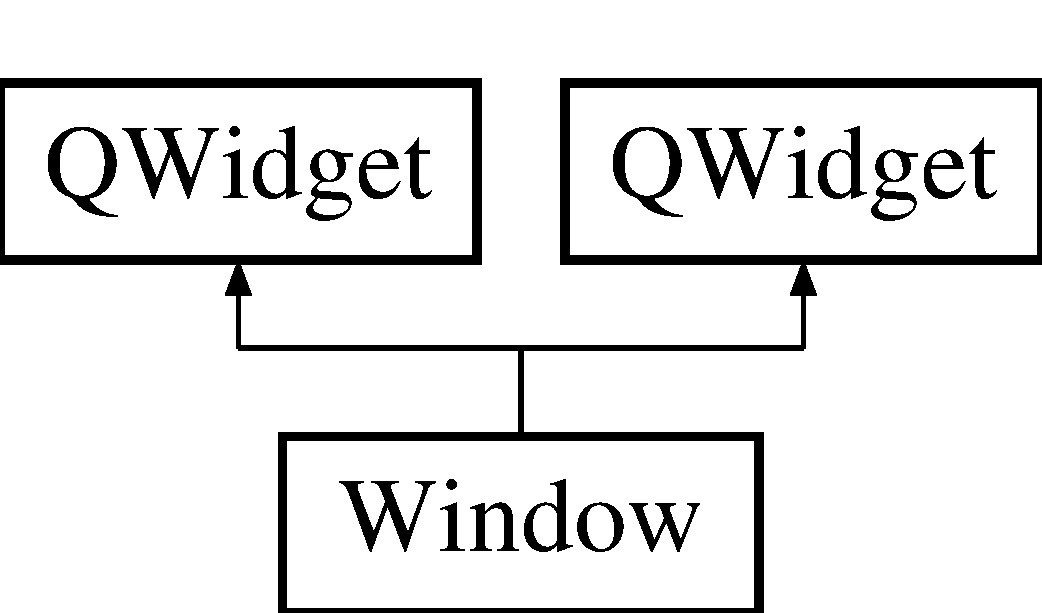
\includegraphics[height=2.000000cm]{classWindow}
\end{center}
\end{figure}
\subsection*{Public Slots}
\begin{DoxyCompactItemize}
\item 
\hypertarget{classWindow_a06531ce47a4206b3dbef30587e768b29}{void {\bfseries set\-Gain} (double gain)}\label{classWindow_a06531ce47a4206b3dbef30587e768b29}

\item 
\hypertarget{classWindow_a06531ce47a4206b3dbef30587e768b29}{void {\bfseries set\-Gain} (double gain)}\label{classWindow_a06531ce47a4206b3dbef30587e768b29}

\end{DoxyCompactItemize}
\subsection*{Public Member Functions}
\begin{DoxyCompactItemize}
\item 
\hypertarget{classWindow_a3656e486c467d9d7c7933812fb4b8f57}{void {\bfseries timer\-Event} (Q\-Timer\-Event $\ast$)}\label{classWindow_a3656e486c467d9d7c7933812fb4b8f57}

\item 
\hypertarget{classWindow_a3656e486c467d9d7c7933812fb4b8f57}{void {\bfseries timer\-Event} (Q\-Timer\-Event $\ast$)}\label{classWindow_a3656e486c467d9d7c7933812fb4b8f57}

\end{DoxyCompactItemize}


The documentation for this class was generated from the following files\-:\begin{DoxyCompactItemize}
\item 
/home/travis/build/a2198699s/pitch-\/perfector/\-Code/fft\-\_\-object/window.\-h\item 
/home/travis/build/a2198699s/pitch-\/perfector/\-Code/fft\-\_\-object/window.\-cpp\end{DoxyCompactItemize}

%--- End generated contents ---

% Index
\newpage
\phantomsection
\addcontentsline{toc}{chapter}{Index}
\printindex

\end{document}
